\subsection{Smoothed Profile Method}
固液二相シミュレーションにおいて,固体-液体の移動境界の取り扱いは非常に重要である.
今回のシミュレーションでは,物理量とは異なる識別関数を導入し,
仮想流体領域を考えるSmoothed Profile Method(SPM)\cite{}を用いた.
SPMでは,流体と粒子の界面にFig.\ref{fig:spm}で表されるような界面関数$\phi$を導入する.
ここで,$a$は粒子の半径,$\xi$は界面の幅を表す.
この界面関数は,流体領域で$\phi=0$,粒子領域で$\phi=1$をとり,
幅$\xi$の界面領域では滑らかに変化する連続関数である.
界面関数の導入により,境界条件を解く必要がなくなり,
計算負荷を軽減され,
以下で説明するNavier-Stokes方程式,
および運動方程式を直接数値計算によって解くことが可能となる.

    \begin{figure}[H]
        \centering
        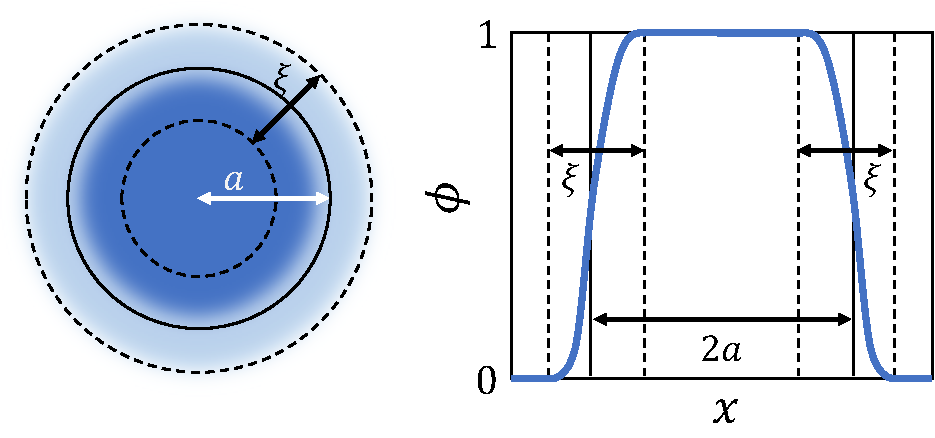
\includegraphics[scale=0.8]{/Users/taiga/Projects/lab/thesis/components/chapter2/figs/spm.pdf}
        \caption{SPMの界面関数}
        \label{fig:spm}
    \end{figure}

